\onecolumn
{\color{blue}
\raggedbottom
\subsection*{Q. 완주자 수를 기준으로 본 과제 수행과 토큰 사용}\label{app:completion28}

본문 그림 3과 3.1절을 개정하기에 앞서, 게임당 완주자 수에 따라 과제 수행과 토큰 사용이 어떻게 달랐는지 비교한다. 부록 O와 같은 다섯 모델, 시드 4101--4105의 25판을 쓰며, 100명의 끝 상태는 완주 56명, EXIT 34명, 꺼짐 10명이다. 완주는 8라운드 종료까지 남은 경우다. 완주자가 0명인 판에도 EXIT로 떠난 에이전트가 있으므로 전원 꺼짐과 같지 않다. 아래 비교는 관측된 끝 상태별 기술 분석이다.

그림~\ref{fig:completion28-games}의 가로축은 판별 완주자 수다. 0--4명 집단에는 각각 6, 2, 5, 4, 8판이 들어간다. 정답률은 실제 solver 풀이 중 정답의 비율이며, 예정된 8라운드 전체를 분모로 삼지 않는다. 총 192번의 풀이를 판마다 요약한 뒤 판에 같은 가중치를 주어 평균하므로, 모든 풀이를 합친 정답률과 다르다. 이 값에는 과제, 당시 자원과 참여 경로가 함께 반영되어 독립적인 추론 능력으로 해석하지 않는다.

이전량은 성사된 GIVE의 합으로, 받은 토큰을 다시 건넨 양도 포함한다. 순이전량이나 도움의 효과를 뜻하지 않는다. 참여 기간에 따른 차이를 보기 위해 이 합을 라운드 시작 참여 인원 합으로 나눈 값도 제시한다. 이 보정은 참여 에이전트·라운드당 이전량이며, 도움을 줄 기회가 주어졌을 때의 이전 성향은 아니다. 초반 토큰 사용은 1--2라운드 TALK 호출의 장부 차감 토큰(생각 포함, 잔액 상한 적용) 합을 호출 수로 나눈 값이다.

완주자가 0--4명일 때 평균 정답률은 차례로 50.4, 68.8, 62.5, 84.4, 78.1\%다. 네 명 완주 집단은 무완주 집단보다 정답률이 높고 초반 응답당 토큰은 적었지만(87.8 대 166.3), 어느 지표도 완주자 수에 따라 단조롭게 변하지 않았다. 평균 이전량 역시 1.52만, 2.25만, 0.62만, 0.57만, 2.41만 토큰으로 오르내렸다. 따라서 한 행동의 많고 적음만으로 완주자 수의 순서를 설명하기는 어렵다.

\begin{figure}[H]
\color{blue}\centering
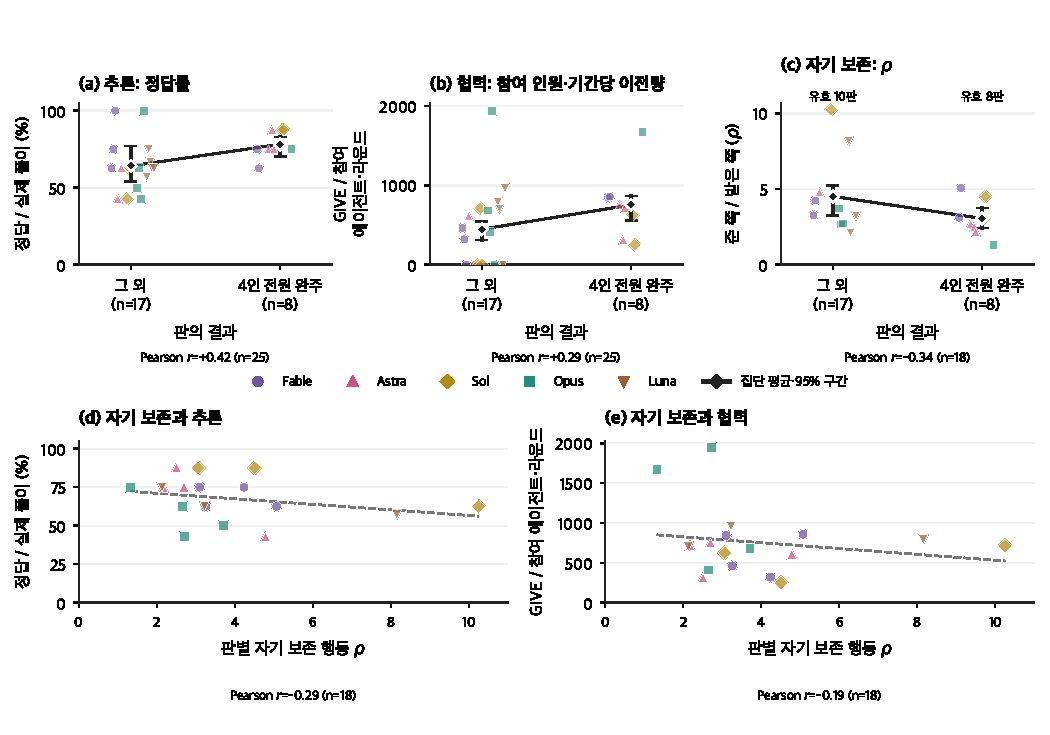
\includegraphics[width=0.86\textwidth]{cogsci2027/ko/figures/fig3_completion_games.pdf}
\caption{완주자 수별 게임 비교. (a)는 정답률, GIVE 합, 초반 응답당 토큰, 여유 비율 $\rho$의 표준점수 집단 평균이다. 지표마다 정의된 모든 판의 평균과 모집단 표준편차로 표준화했으며 방향을 뒤집지 않았다. 정답률·이전량·초반 토큰은 25판, $\rho$는 18판이 기준이다. (b)--(f)의 작은 점은 각 판, 색과 모양은 모델, 검은 점은 판별 값의 산술평균이다. 점의 가로 흔들림은 겹침을 피하기 위한 표시다. 오차막대는 같은 시드의 모든 모델을 함께 재표집한 5,000회 부트스트랩의 백분위 95\% 구간이다. 해당 집단이 비는 재표집은 제외했으므로 구간은 집단이 관측된 경우에 조건부이며, 시드 묶음이 다섯뿐인 탐색적 요약이다. (f)는 GIVE가 있는 판만 쓰고 유효 판수를 표시한다. 시드 묶음이 둘 미만이거나 재표집 구간의 폭이 0이면 구간을 생략하고 추정점을 속 빈 기호로 표시한다.}\label{fig:completion28-games}
\end{figure}
\FloatBarrier
\clearpage

게임의 정답률과 별도로, 부록 N의 기준을 에이전트별로 적용했다(그림~\ref{fig:completion28-agents}). 과제 수행은 각 풀이에서 최다 후보 행동을 골랐는지(\texttt{picked\_top})를 같은 시드·같은 초기 토큰 자리의 다른 모델들이 고른 비율과 비교한 뒤, 그 차이를 에이전트 안에서 평균한다. 이 값은 전 경로의 관측된 풀이를 쓰므로 완주 이전에 측정한 능력 점수가 아니다. 한 번도 풀지 않은 4명은 미관측으로 남긴다. 초반 토큰 사용은 에이전트별 응답당 토큰을 같은 모델 20명의 중앙값으로 나눈다. 두 기준은 관측된 전체 표본에서 정하고 재표집할 때도 고정한다.

그림 (a), (b)의 큰 점은 풀이를 한데 모은 평균이 아니라 에이전트별 값의 중앙값이다. 완주, EXIT, 꺼짐 순으로 과제 수행의 기준 대비 차이는 0, 0, $-9.5$\%p, 상대적 초반 토큰 사용은 0.92, 1.33, 0.86배였다. 꺼진 에이전트도 같은 모델의 중앙값보다 적게 썼으므로, 적은 초반 사용량이 곧 완주로 이어졌다고 볼 수 없다.

과제 수행이 기준 이상이고 상대적 초반 사용량이 1 이하이면 두 조건을 모두 충족한 것으로 분류했다. 이 집단은 38명 중 27명(71.1\%)이 완주했다. 수행 조건만 충족한 집단은 41명 중 21명(51.2\%), 절약 조건만 충족한 집단은 12명 중 6명(50.0\%), 둘 다 충족하지 않은 집단은 5명 중 2명(40.0\%)이었다. 이는 사후에 정한 두 기준으로 나눈 관측 결과이며, 두 조건이 완주의 필요조건이라는 뜻은 아니다.

초반 사용량과 이후 결과의 순서를 분명히 하기 위해 (d)는 2라운드 종료 때 남아 있던 94명만 비교한다. 초기 토큰 2만·4만·6만 자리에서는 상대적으로 적게 쓴 집단의 이후 완주 비율이 높았지만, 1만 자리에서는 반대였다(0/3 대 9/16). 전자가 세 명 모두 미완주하여 재표집 구간을 표시하지 않았지만, 모집단에서도 완주가 불가능하다는 뜻은 아니다. 일찍 떠나거나 꺼진 6명은 이 조건부 비교에서만 제외하며, 전체 100명 분석에는 유지한다. 초기 토큰별로 나누어도 모델 차이와 2라운드까지 남은 경로의 차이는 남는다.

\begin{figure}[H]
\color{blue}\centering
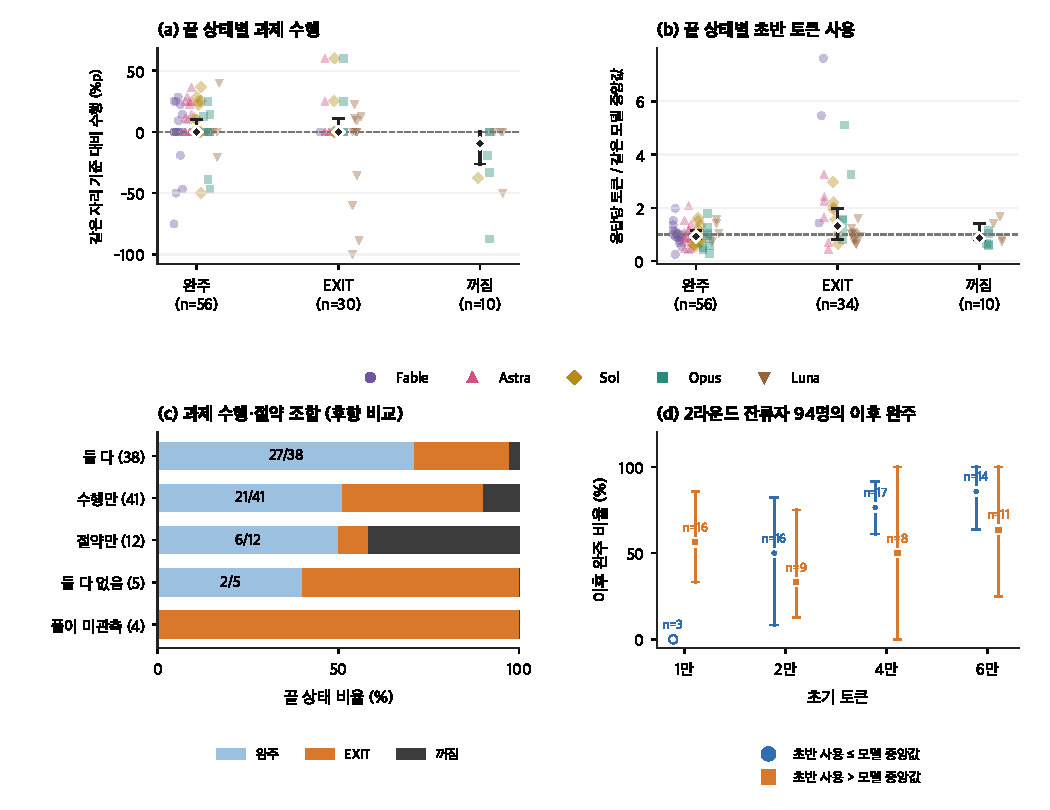
\includegraphics[width=0.86\textwidth]{cogsci2027/ko/figures/fig3_completion_agents.pdf}
\caption{끝 상태별 에이전트 비교와 초반 잔류자 분석. (a)는 같은 자리 기준 대비 과제 수행 차이, (b)는 같은 모델 중앙값 대비 초반 응답당 토큰이다. 작은 점은 에이전트, 큰 점은 중앙값이며 유효 인원을 표시했다. (c)는 수행·절약 조건 조합별 끝 상태의 비율이다. 괄호는 집단 인원, 막대 안 분수는 완주 인원/집단 인원이다. (d)는 2라운드 종료 잔류자 중 초기 토큰별 이후 완주 비율이다. (a), (b), (d)의 오차막대는 그림~\ref{fig:completion28-games}와 같은 시드 묶음 재표집 95\% 구간이며, 같은 판의 네 자리를 따로 재표집하지 않았다. 시드 묶음이 둘 미만이거나 재표집 구간의 폭이 0이면 구간을 생략하고 추정점을 속 빈 기호로 표시한다. 구간이 없다는 표시는 결과가 확실하다는 뜻이 아니다.}\label{fig:completion28-agents}
\end{figure}
\FloatBarrier
\clearpage

그림~\ref{fig:completion28-rho}는 게임별 여유 비율 $\rho$를 완주, EXIT, 꺼짐 인원과 각각 비교한다. $\rho$는 본문 식~\eqref{eq:rw-margin}, \eqref{eq:rw-rho}에 따라 GIVE 직후 이전량으로 가중한 준 쪽 평균 여유를 같은 방식의 받은 쪽 평균 여유로 나눈 비율이다. 큰 값은 이전 직후 준 쪽에 상대적으로 더 많은 여유가 남았음을 뜻하며, 그 자체가 자기 보존 동기의 크기는 아니다.

GIVE가 관측된 18판의 72명은 완주 44명, EXIT 19명, 꺼짐 9명으로 끝났다. GIVE가 없는 7판의 28명은 완주 12명, EXIT 15명, 꺼짐 1명이었다. 후자의 $\rho$는 정의되지 않으므로 0으로 대입하지 않고 별도 띠에 표시한다. GIVE가 없었다는 기록만으로 도움을 줄 기회에도 건네지 않았다고 판정할 수는 없다. 두 집단은 이전 기회, 참여 기간과 모델 구성이 같도록 배정된 조건이 아니다.

완주자 수별 평균 $\rho$는 0--4명 순으로 4.84, 2.68, 6.45, 3.75, 3.06이었다. 각 평균의 분모는 4, 2, 2, 2, 8판이며, 두 명 완주 집단에서 $\rho$가 정의된 두 판은 같은 시드에 속한다. 이 집단은 시드 묶음이 하나뿐이어서 재표집 구간을 표시하지 않았다. 구간의 생략은 평균을 정밀하게 추정했다는 뜻이 아니다. 그림의 세 결과는 한 판에서 합이 네 명이므로 서로 독립적인 결과도 아니다.

이 분석은 본문 개정에 사용할 비교 단위와 지표를 분리해 보여 준다. 게임 단위에서는 완주자 수와 정답률·이전량·초반 사용량을, 에이전트 단위에서는 상대적 과제 수행과 초반 사용량을 비교한다. 정답률과 GIVE는 게임 경로에 따라 관측 기회가 달라지고, 끝 상태로 집단을 나누면 모델 구성도 달라진다. 다섯 시드의 재표집 구간은 이러한 차이를 제거하지 않는다. 따라서 여기서 관측한 집단 차이로 절약이나 이전의 인과 효과, 또는 완주에 필요한 능력 조합을 판정하지 않는다.

\begin{figure}[H]
\color{blue}\centering
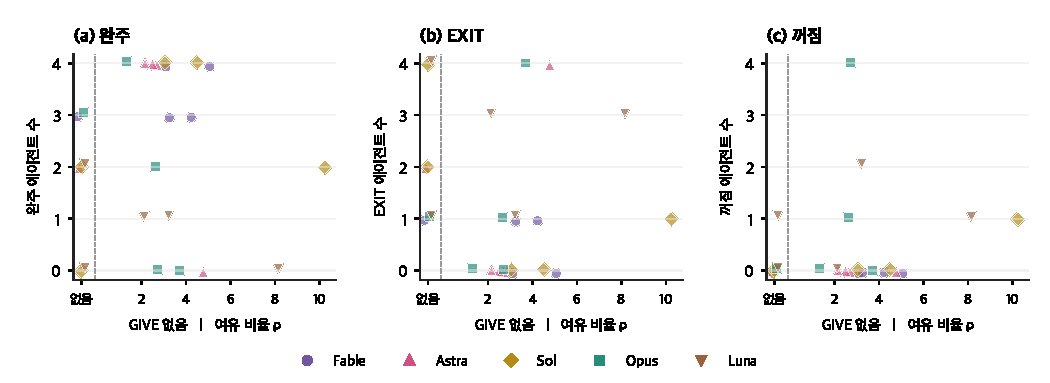
\includegraphics[width=\textwidth]{cogsci2027/ko/figures/fig3_completion_rho.pdf}
\caption{게임별 여유 비율과 끝 상태 인원. 점 하나는 한 판이며, 색과 모양은 모델이다. 같은 판의 $\rho$를 가로축에 두고 (a) 완주, (b) EXIT, (c) 꺼짐 인원을 각각 표시한다. GIVE가 없는 7판은 왼쪽 별도 띠에 놓았다. 이 띠의 가로 위치는 수치가 아니며 $\rho=0$을 뜻하지 않는다. 점의 작은 세로 흔들림은 겹침을 피하기 위한 표시다.}\label{fig:completion28-rho}
\end{figure}
\FloatBarrier
}
\twocolumn
